%package list
\documentclass{article}
\usepackage[top=3cm, bottom=3cm, outer=3cm, inner=3cm]{geometry}
\usepackage{graphicx}
\usepackage{url}
%\usepackage{cite}
\usepackage{hyperref}
\usepackage{array}
%\usepackage{multicol}
\newcolumntype{x}[1]{>{\centering\arraybackslash\hspace{0pt}}p{#1}}
\usepackage{natbib}
\usepackage{pdfpages}
\usepackage{multirow}
\usepackage{multirow}
\usepackage[T1]{fontenc}
\usepackage{imakeidx}
% Imagenes de costado
\usepackage{wrapfig}
\usepackage{graphicx}

% Modificar URLs
\usepackage{hyperref}
\hypersetup{
    colorlinks=true,
    linkcolor=black,
    filecolor=magenta,      
    urlcolor=blue,
    pdftitle={Overleaf Example},
    pdfpagemode=FullScreen,
    }

\urlstyle{same}


\usepackage[normalem]{ulem}
\useunder{\uline}{\ul}{}

\usepackage{minted}

% codigo fuente
\usepackage{listings}
\usepackage{color, colortbl}
\definecolor{dkgreen}{rgb}{0,0.6,0}
\definecolor{gray}{rgb}{0.5,0.5,0.5}
\definecolor{mauve}{rgb}{0.58,0,0.82}
\definecolor{codebackground}{rgb}{0.95, 0.95, 0.92}
\definecolor{tablebackground}{rgb}{0.0, 0.45, 0.63}
\lstset{frame=tb,
	language=bash,
	aboveskip=3mm,
	belowskip=3mm,
	showstringspaces=false,
	columns=flexible,
	basicstyle={\small\ttfamily},
	numbers=none,
	numberstyle=\tiny\color{gray},
	keywordstyle=\color{blue},
	commentstyle=\color{dkgreen},
	stringstyle=\color{mauve},
	breaklines=true,
	breakatwhitespace=true,
	tabsize=3,
	backgroundcolor= \color{codebackground},
}

%%%%%%%%%%%%%%%%%%%%%%%%%%%%%%%%%%%%%%%%%%%%%%%%%%%%%%%%%%%%%%%%%%%%%%%%%%%%
%%%%%%%%%%%%%%%%%%%%%%%%%%%%%%%%%%%%%%%%%%%%%%%%%%%%%%%%%%%%%%%%%%%%%%%%%%%%
\newcommand{\csemail}{vmachacaa@ulasalle.edu.pe}
\newcommand{\csdocente}{MSc. Maribel Molina Barriga}
\newcommand{\cscurso}{Sistemas Operativos}
\newcommand{\csuniversidad}{Universidad La Salle}
\newcommand{\csescuela}{Escuela Profesional de Ingeniería de Software}
\newcommand{\cspracnr}{01}
\newcommand{\cstema}{Instalación Debian}
%%%%%%%%%%%%%%%%%%%%%%%%%%%%%%%%%%%%%%%%%%%%%%%%%%%%%%%%%%%%%%%%%%%%%%%%%%%%
%%%%%%%%%%%%%%%%%%%%%%%%%%%%%%%%%%%%%%%%%%%%%%%%%%%%%%%%%%%%%%%%%%%%%%%%%%%%


\usepackage[english,spanish]{babel}
\usepackage[utf8]{inputenc}
\AtBeginDocument{\selectlanguage{spanish}}
\renewcommand{\figurename}{Figura}
\renewcommand{\refname}{Referencias}
\renewcommand{\tablename}{Tabla} %esto no funciona cuando se usa babel
\AtBeginDocument{%
	\renewcommand\tablename{Tabla}
}

\usepackage{fancyhdr}
\pagestyle{fancy}
\fancyhf{}
\setlength{\headheight}{30pt}
\renewcommand{\headrulewidth}{1pt}
\renewcommand{\footrulewidth}{1pt}
\fancyhead[L]{\raisebox{-0.2\height}{
\includegraphics[width=3cm]{logo_ulasalle (1).png}}}
\fancyhead[C]{}
\fancyhead[R]{\fontsize{7}{7}\selectfont	\csuniversidad \\ \csescuela \\ \textbf{\cscurso} }
\fancyfoot[L]{}
\fancyfoot[C]{Sistemas Operativos}
\fancyfoot[R]{Página \thepage}



\begin{document}

	\vspace*{10px}
	
	\begin{center}	
		\fontsize{17}{17} \textbf{ Práctica \cspracnr}
	\end{center}
	%\centerline{\textbf{\underline{\Large Título: Informe de revisión del estado del arte}}}
	%\vspace*{0.5cm}
	

\renewcommand{\arraystretch}{1.5}
\begin{table}[h]
	\begin{tabular}{|x{4.7cm}|x{4.8cm}|x{4.8cm}|}
		\hline 
		\textbf{DOCENTE} & \textbf{CARRERA}  & \textbf{CURSO}   \\
		\hline 
		\csdocente & \csescuela & \cscurso    \\
		\hline 
	\end{tabular}
\end{table}	

\begin{table}[h]
	\begin{tabular}{|x{4.7cm}|x{4.8cm}|x{4.8cm}|}
		\hline 
		\textbf{GRUPO} & \textbf{TEMA}  & \textbf{DURACIÓN}   \\
		\hline 
		\ 6 & \cstema & 5 horas   \\
		\hline 
	\end{tabular}
\end{table}
\renewcommand{\arraystretch}{1} 
	\section*{Integrantes}
	 	\begin{itemize}
                    \item José Carlos Machaca Vera
	 		\item Jhosep Alonso Mollapaza Morocco
	 		\item Patrick Andres Ramirez Santos
	 \end{itemize}
 
	\tableofcontents


	

\newpage

\section{Instalación Debian minimal}
    \subsection{Oracle VirtualBox}
        Se instala el programa de virtualización VirtualBox en una computadora con dual boot de Fedora 39 y Windows 11, especificamente en Fedora. Se siguieron los siguientes pasos:
        \begin{enumerate}
            \item Descargar VirtualBox de la pagina de descargas oficial
            \item Intalar el programa 
            \item Descargar ISO Debian 12 
        \end{enumerate}
        

        Luego se configura una nueva máquina virtual para instalar la version mínima de Debian, la instalación completa puede encontrarse \href{https://youtu.be/oMSiG6R_-X8}{aquí}: \\ 
    
    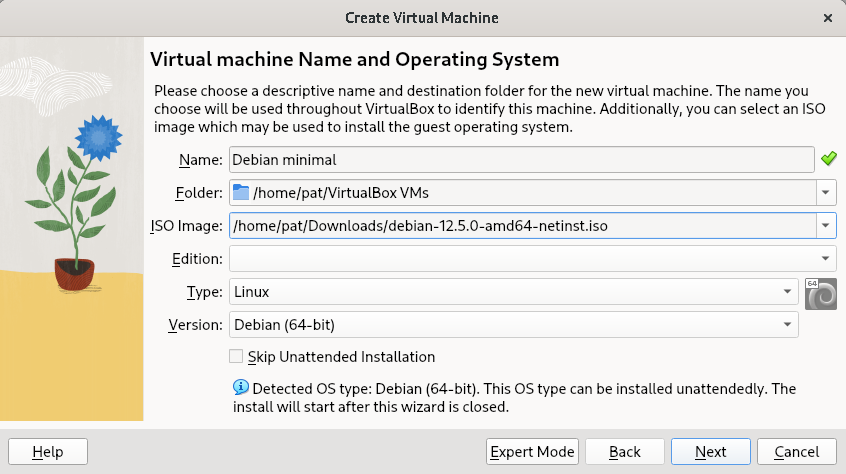
\includegraphics[scale=0.5]{capturas_debian/VM-init.png}

    \subsection{Paquetes}
        Una vez instalada la version minima se ingresa con el super usuario, en nuestro caso sudo no estaba disponible y se procedió a instalar el paquete para luego poder añadir el resto de paquetes con facilidad. Ademas se instaló el paquete build-essential (incluye los compiladores de C y C++) , Git, Neovim (se utilizará en vez de Vim debido a la facilidad de configuracion), Vim y Openjdk. Finalmente se verifica la existencia de los paquetes requeridos:
        \begin{minted}{bash}
        $ su rooot
        $ apt install sudo
        $ sudo apt install git vim neovim openjdk-17-jdk build-essentials -y
        $ dpkg -l git vim openjdk-17-jdk gcc g++
        \end{minted}

        Los resultados de la instalación pueden obervarse en la siguiente imagen:
        
        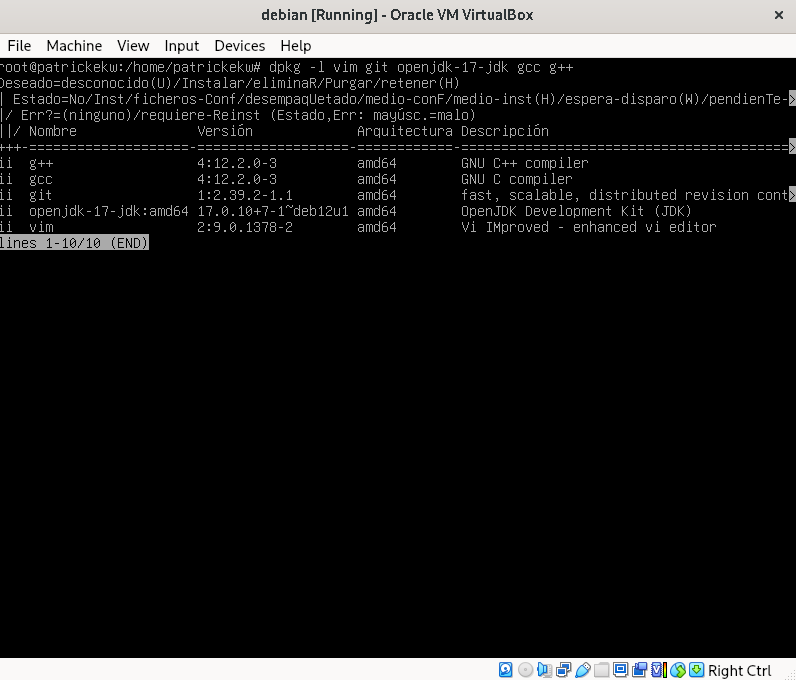
\includegraphics[scale=0.5,trim={0 15cm 0 0},clip]{capturas_debian/Paquetes.png}  


\section{Debian UI con Plasma}
Para la segunda parte de la práctica se pide instalar aplicaciones que requieres una interfaz gráfica de usuario, para nuestro caso decidimos utilizar KDE Plasma, instalando el paquete luego seleccionando las preferencias y finalizando con un reboot del sistema de la siguiente forma:
    \begin{minted}{bash}
        $ sudo apt install kde-plasma-desktop
        $ sudo reboot
    \end{minted}

%\begin{center}
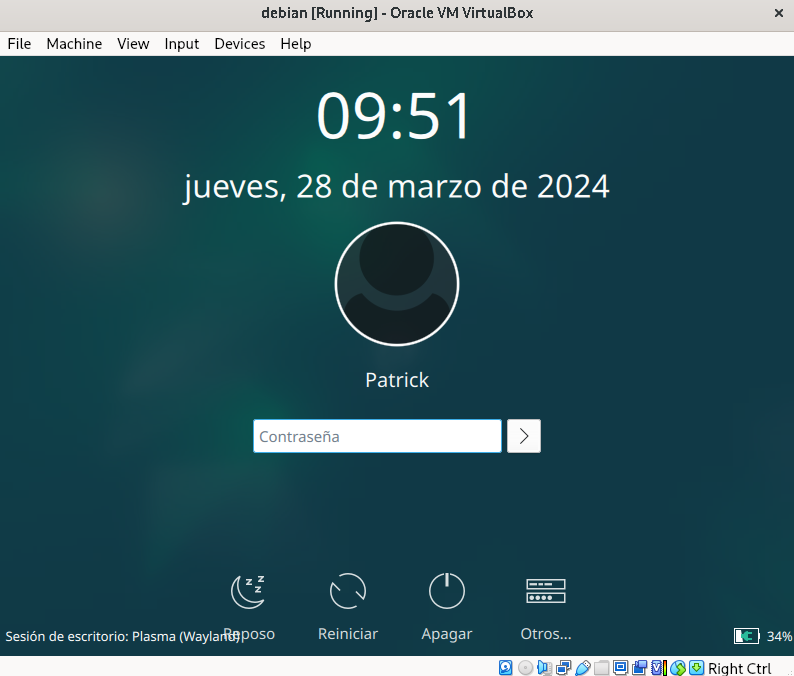
\includegraphics[scale=0.5]{capturas_debian/Plasma.png}  
% \end{center}
    \subsection{Visual Studio Code}
    Nos dirigimos a la pagina oficial de descargas de Visual Studio Code y descargamos la version .deb para arm64 en Linux, luego nos ubicamos en el folder con el archivo y lo instalamos usando la terminal, se puede visualizar el programa en la imagen debajo de los comandos:
    \begin{minted}{bash}
        $ cd Descargas
        $ su root
        $ sudo dpkg -i code_1.87.2-1709911730_arm64.deb
    \end{minted}

    \subsection{Sublime Text Editor}
    Se instala Sublime, primero descargamos e instalamos la clave GPG y se instala para apt, luego se indica a Debian que APT puede descargar Sublime de la URL proporcionada, por ultimo se actualizan los paquetes anteriores y se instala Sublime con APT. Todos estos pasos estan descritos en la documentacion de \href{https://www.sublimetext.com/docs/linux_repositories.html#apt}{Sublime}:
    \begin{minted}[tabsize=2,breaklines]{bash}
        $ wget -qO - https://download.sublimetext.com/sublimehq-pub.gpg | gpg --dearmor | sudo tee \\ /etc/apt/trusted.gpg.d/sublimehq-archive.gpg > /dev/null
        $ echo "deb https://download.sublimetext.com/ apt/stable/" | sudo tee /etc/apt/sources.list.d/sublime-text.list
        $ sudo apt-get update
        $ sudo apt-get install sublime-text
    \end{minted}
    \subsection{Notepad++}
    Notepad++ no tiene una build nativa para Linux, pero se puede instalar utilizando snaps que a su vez implementan wine para simular un entorno de Windows, para ello se instaló el paquete y luego se abrio la aplicación desde la terminal con los siguientes comandos:

    \begin{minted}[tabsize=2,breaklines]{bash}
        $ sudo apt install snapd
        $ sudo systemctl enable snapd
        $ sudo systemctl start snapd
        $ sudo snap install notepad-plus-plus
        $ snap run notepad-plus-plus
    \end{minted}

    \subsection{Vim}
    Por último al ya haber instalado Vim en la sección de instalación miníma se decidió añadir la configuración \href{https://github.com/theopn/kickstart.vim}{kickstart} que incluye carios paquetes y configuración preinstalada. Para ello se conectó la repo de Github a Vim mediante un link simbólico. Finalmente se abre desde la terminal con la nueva configuración:
    
    \begin{minted}[tabsize=2,breaklines]{bash}
        $ git clone https://github.com/theopn/kickstart.vim.git ~/kickstart.vim
        $ ln -sf ~/kickstart.vim/.vimrc ~/.vimrc
        $ vim
    \end{minted}    

    \newpage

    Finalmente se puede visualizar la interfaz grafica de los programas descritos: \\
    
        \begin{tabular}{cc}
        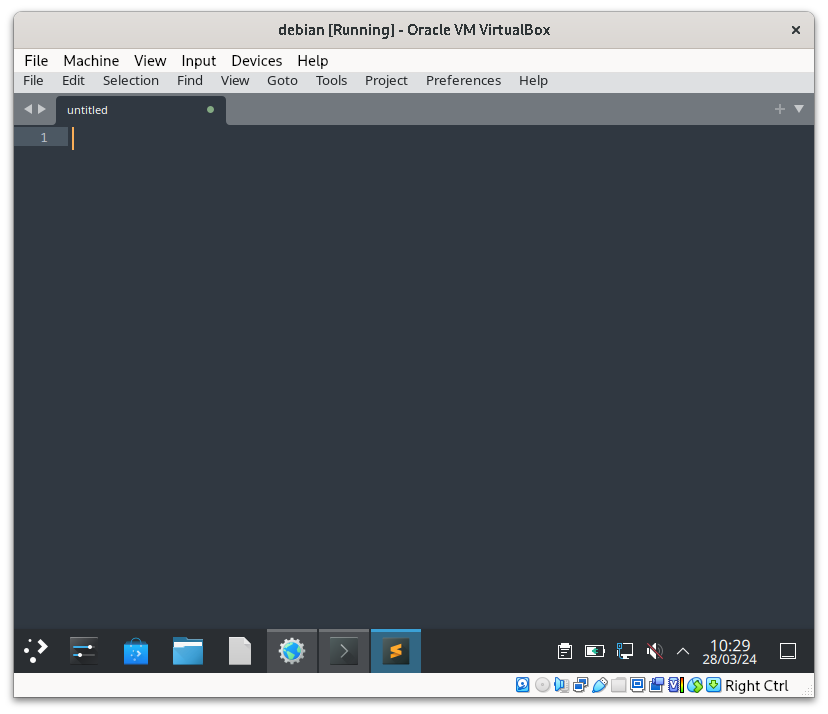
\includegraphics[width=.4\linewidth,valign=m]{capturas_paquetes/sublime.png} & 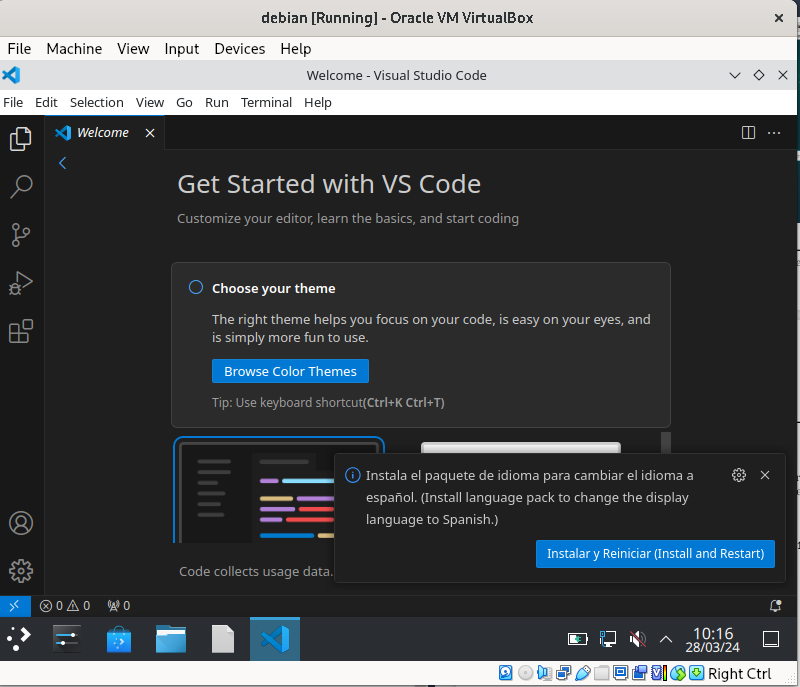
\includegraphics[width=.4\linewidth,valign=m]{capturas_paquetes/vscode.png} \\
        Sublime & VS Code \\
        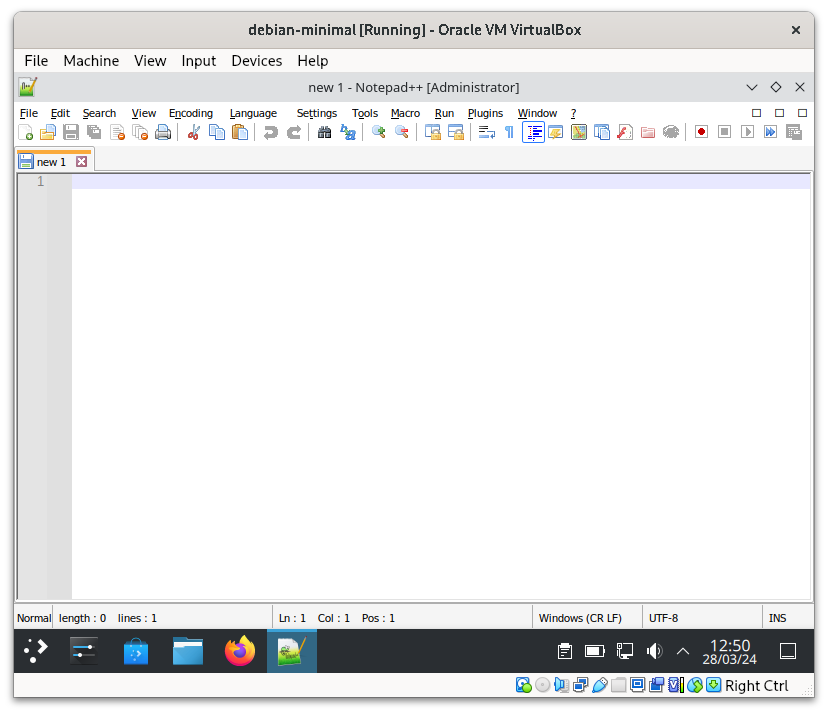
\includegraphics[width=.4\linewidth,valign=m]{capturas_paquetes/notepad.png} & 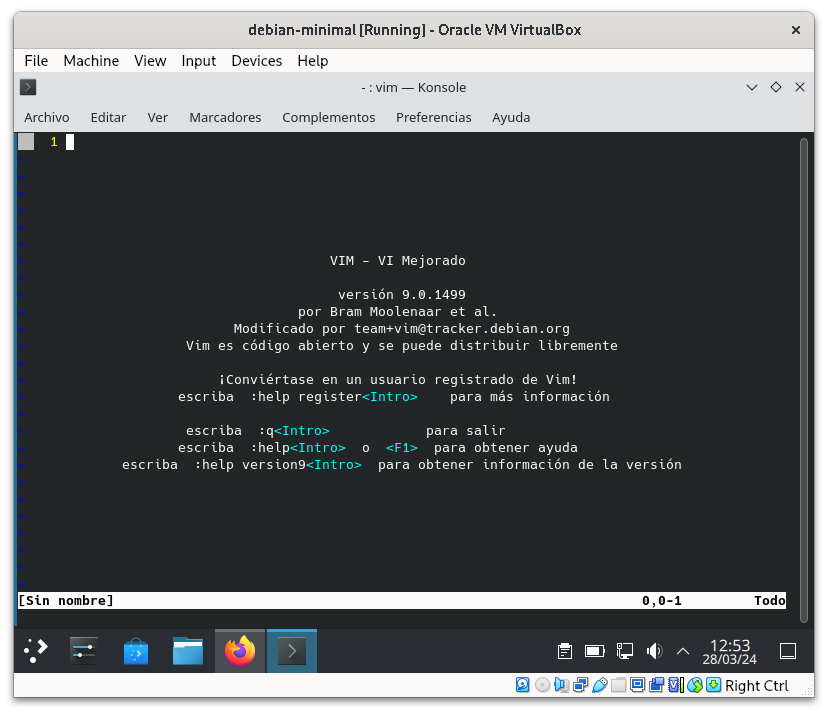
\includegraphics[width=.4\linewidth,valign=m]{capturas_paquetes/vim.png} \\
        Notepad++ & Vim \\
    \end{tabular}

\section{Conclusiones}
    \begin{itemize}
        \item Existen varias formas de instalar programas en Debian, muchas se pueden hacer desde la terminal pero tambien existen instaladores como snap.
        \item Los comandos apt-get y apt funcionan de forma similar, siendo el último una versión mas reciente
        \item Instalar una GUI para Linux puede ser un proceso relativamente sencillo que no requiere mucha configuración si se utiliza los paquetes correctos.
    \end{itemize}
    


	%\clearpage
	%\bibliographystyle{apalike}
	%\bibliographystyle{IEEEtranN}
	%\bibliography{bibliography}
		
	
\end{document}
